% 日本語で文書を作る設定
% タイトル・概要ページ付き
\documentclass[titlepage]{jlreq}

% PCで見るように自動リンク
\usepackage{hyperref}

% hyperrefを使ってrefの種類を自動判別して接頭辞をつける
\def\equationautorefname~#1\null{\textrm{~(#1)式\;}\null}
\def\figureautorefname~#1\null{ 図~#1\null}
\def\tableautorefname~#1\null{ 表~#1\null}
\def\sectionautorefname~#1\null{第~#1章\null}
\def\subsectionautorefname~#1\null{~#1節\null}
\def\subsubsectionautorefname~#1\null{~#1節\null}
\def\paragraphautorefname~#1\null{第~#1パラグラフ\null}
\def\subparagraphautorefname~#1\null{第~#1小パラグラフ\null}
\def\pageautorefname~#1\null{~#1ページ \null}
\def\appendixautorefname~#1\null{~#1 \null}
% 参照のショートカット
\newcommand\aref[1]{\autoref{#1}}

% 画像貼り付け
\usepackage{graphicx}

% その位置に指定して置く
\usepackage{float}

% タイトル・著者の使いまわし
\usepackage{authoraftertitle}

% 化学構造式(きれいに書く方)
\usepackage{xymtexps}

% 図表を次のsectionにおかないように設定
\usepackage[section]{placeins}

% 複数行の数式を書く
\usepackage{amsmath}

% ≒を使う
\usepackage{amssymb}

% セクションにドットをつける (1 見出し → 1. 見出し)
\usepackage{secdot}
\sectionpunct{section}{.}
\sectionpunct{subsection}{}
\sectionpunct{subsubsection}{}
\sectionpunct{paragraph}{}
\sectionpunct{subparagraph}{}

% 問題なくキャプションは使えるが警告が出るため黙らせる
\usepackage{silence}
\WarningFilter{caption}{Unknown document}
% キャプションを設定
\usepackage{caption}
\usepackage{varwidth}
% 中央寄せをデフォルトにしたスタイルを作成
\DeclareCaptionFormat{capfmt}{%
  % #1: label (e.g. "Table 1")
  % #2: separator (e.g. ": ")
  % #3: caption text
  \begin{varwidth}{\linewidth}%
    \centering
    #1#2#3%
  \end{varwidth}%
}

% SI単位系を扱う
\usepackage{siunitx}
% \SI{数値}{単位}で表示できるが、
% {数値}にxのような変数を入れるためのコマンド\SIeqを定義
\newcommand{\SIeq}[2]{\SI[parse-numbers=false]{#1}{#2}}

% ソースコード添付用
% 日本語コメントに対応したjvlistingを使用
\usepackage{listings,jvlisting} 
\lstset{
  basicstyle={\ttfamily},
  identifierstyle={\small},
  commentstyle={\small},
  keywordstyle={\small\bfseries},
  ndkeywordstyle={\small},
  stringstyle={\small\ttfamily},
  frame={tb},
  breaklines=true,
  columns=[l]{fullflexible},
  numbers=left,
  xrightmargin=0em,
  xleftmargin=3em,
  numberstyle={\scriptsize},
  stepnumber=1,
  numbersep=1em,
  lineskip=-0.5ex
}

% 参考文献の参照を上付きに
\usepackage[super]{cite}

\begin{document}

% キャプションの設定
% 作ったスタイルを割り当て
\captionsetup{format=capfmt}
% 番号と見出しの区切りを空白に
\captionsetup{labelsep=quad}

\makeatletter
    % abstractを通常のsectionと同様に変更
    \renewenvironment{abstract}{%
    \titlepage
    \@beginparpenalty\@lowpenalty\noindent
    {\Large\bfseries\abstractname}\\%
    \@endparpenalty\@M
    }%
    {\par\endtitlepage}
    \renewcommand{\abstractname}{要旨}

    % 太横線を定義
    \def\Hline{
        \noalign{\ifnum0=`}\fi\hrule \@height 4.\arrayrulewidth \futurelet
        \reserved@a\@xhline}
    
    % ソースコードのキャプション見出しを変更
    \renewcommand{\lstlistingname}{コード}

    % 参考文献の参照を <x)> の形式に変更
    \renewcommand\citeform[1]{#1)}

    % 参考文献のリストの見出しを <x)> の形式に変更
    \def\@biblabel#1{#1)}
\makeatother

% \\で改行。もうちょっと空白欲しいから二重に改行
% %がないと段落になって一文字下がるから注意
\title{%
    レポートタイトル1行目
    \\\\
    レポートタイトル2行目
    }

% 作者の名前を入れる
\author{S.T.}

% 表紙を作る
% もろもろは直打ち。

\begin{titlepage}

    \vspace*{60pt} \noindent
    {\LARGE 2024 年} 
    \vspace{14pt} \\
    {\LARGE example レポート} 
    \vspace{100pt} \\
    {\Large \MyTitle}
    \vspace{130pt} \\
    \begin{tabular}{ll}
        提出者     & A番 \MyAuthor  \\
        実験日     & 令和 R 年 m 月 d 日(D) \\
        提出日     & 令和 R 年 m 月 d 日(D) \\
        共同実験者 & A番 X.Y. \\
                   & A番 V.W. \\
    \end{tabular} \vspace{3pt} \\
\end{titlepage}

\begin{abstract}

ここに要旨を書く。
このページはページ番号が割り振られない。
中央寄せを解除し、他の章と同じような見た目にしている。

\end{abstract} 


\section{目的}

目的を記載する。

\section{実験器具}

\subsection{環境}

\begin{itemize}
    \item PC
    \item vscode
    \item TexLive2022
\end{itemize}

\section{実験方法}

実験方法を記載する。

\section{実験結果}

実験結果を記載する。

\section{考察}

考察を記載する。

表は\aref{tbl:example}のように記載する

\begin{table}[H]
    \centering
    \caption{表の例}
    \label{tbl:example}
    \begin{tabular}{ccc}
        \Hline
        1 & 2 & 3
        \\\Hline
    \end{tabular}
\end{table}


図は\aref{fig:ex1}のように記載する

\begin{figure}[H]
    \centering
    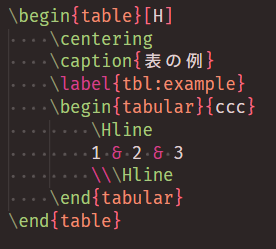
\includegraphics[width=0.8\linewidth]{simple-chem-report.tex_assets/fig1.png}
    \caption{図の貼り付けの例}
    \label{fig:ex1}
\end{figure}

ソースコードは\aref{code:ex1}のように記載する

\begin{lstlisting}[
    caption=ソースコード貼り付けの例,
    label=code:ex1
]
\begin{figure}[H]
    \centering
    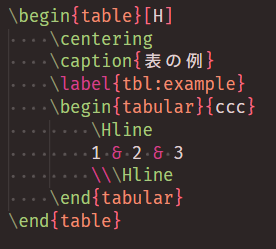
\includegraphics[width=0.8\linewidth]{simple-chem-report.tex_assets/fig1.png}
    \caption{図の貼り付けの例}
    \label{fig:ex1}
\end{figure}
\end{lstlisting}

化学構造図は\aref{fig:penta}のように書く

\begin{figure}[H]
    \centering
    \pentamethylene{1==a1;2==a2;3==a3;4==a4;5==a5}%
    {1==1;2==2;3==3;4==4;5==5}
    \bzdrv{1==1;2==2;3==3;4==4;5==5;6==6}
    \caption{化学構造図の例 兼結合数字の位置}
    \label{fig:penta}
\end{figure}


pentamethyleneの3とbzdrvの1をつなぐと\aref{fig:p3bz1}のようになる。
一番長い鎖が最初に来るように書くこと。また、ベンゼンは後になる。
重なって邪魔になる部分は消去した。

pentamethyleneの3の腕とbzdrvの1の腕が重なり合うという意味の書き方。
pentamethyleneの3に直接bzdrvを書き、bzdrvの1の腕に受け取る意味の(yl)を書く

\begin{figure}[H]
    \centering
    \pentamethylene{1==a1;2==a2;3==a3;4==a4;5==a5}%
    {2==2;4==4;3==%
    \bzdrv{1==(yl);2==2;3==3;4==4;5==5;6==6}}
    \vspace*{2cm}
    \caption{pentamethyleneの3とbzdrvの1をつなぐ}
    \label{fig:p3bz1}
\end{figure}

繋がる個数によって接頭辞がつく。
hexa(6)以上は(yl)を使用してつなぎ合わせて作る。

\[
    \centering
    \begin{tabular}{ll}
        \Hline
        接頭辞 & 個数
        \\\Hline
        di & 2\\
        try & 3\\
        tetra & 4\\
        penta & 5\\
        hexa & 6
        \\\Hline
    \end{tabular}
\]

接尾辞は次のような意味

\[
    \centering
    \begin{tabular}{llll}
        \Hline
        接尾辞 & 省略元 & 意味 & 例
        \\\Hline
        v & vertical   & 垂直方向  & bzdrv\\
        h & horizontal & 水平方向  & bzdrh\\
        i & inverse    & 逆向き    & trimethylenei
        \\\Hline
    \end{tabular}
\]

\begin{align*}
    bzdrv
    &&
    bzdrh
    &&
    trimethylene
    &&
    trimethylene
    \\
    \bzdrv{}
    &&
    \bzdrh{}
    &&
    \trimethylene{1==a1;2==a2;3==a3}{1==1;2==2;3==3}
    &&
    \trimethylenei{1==a1;2==a2;3==a3}{1==1;2==2;3==3}
\end{align*}


ジグザグ形状はmethylene。

\begin{align*}
    dimethylene
    &&
    trimethylene
    &&
    tetramethylene
    \\
    \dimethylene{1==a1;2==a2}{1==1;2==2}
    &&
    \trimethylene{1==a1;2==a2;3==a3}{1==1;2==2;3==3}
    &&
    \tetramethylene{1==a1;2==a2;3==a3;4==4a}{1==1;2==2;3==3;4==4}
\end{align*}

\begin{align*}
    pentamethylene
    &&
    hexamethylene
    \\
    \pentamethylene{1==a1;2==a2;3==a3;4==4a;5==5a}{1==1;2==2;3==3;4==4;5==5}
    &&
    \hexamethylene{1==a1;2==a2;3==a3;4==4a;5==5a;6==6a}{1==1;2==2;3==3;4==4;5==5;6==6}
\end{align*}

trigonal

\begin{align*}
    dtrigonal
    &&
    utrigonal
    \\
    \dtrigonal{0==0;1==1;2==2;3==3}
    &&
    \utrigonal{0==0;1==1;2==2;3==3}
\end{align*}

腕にxSa,xSbと指定すると垂直方向を示せる。

$$
\bzdrv{1Sa==1Sa;1Sb==1Sb;2Sa==2Sa;2Sb==2Sb;3Sa==3Sa;3Sb==3Sb;4Sa==4Sa;4Sb==4Sb;4Sa==4Sa;4Sb==4Sb;5Sa==5Sa;5Sb==5Sb;6Sa==6Sa;6Sb==6Sb;}
$$

英語数字(n)fuseで(n)の輪を結合できる。

\begin{align*}
    &&
    threefuse
    &&
    fourfuse
    &&
    fivefuse
    &&
    sixfuse
    &&
    \\
    &&
    \threefusev{}{}{}
    &&
    \fourfuse{}{}{}
    &&
    \fivefusev{}{}{}
    &&
    \sixfusev{}{}{}
    &&
\end{align*}

\begin{XyMcompd}(1200,300)(250,200){cpd:cycpro3}{etst}
    \cyclopropaneh{1Sa==%
    \ryl(4==CO){4==\tetrahedral{2==(yl);0==CH;1==\ChemForm{COCH_{3}};%
    4==\ChemForm{COOC_{2}H_{5}}}};1Sb==\ChemForm{CH_3}}
\end{XyMcompd}

\begin{XyMcompd}(1000,850)(-150,-150){}{}
    \Ethylenev{1==C;2==N}{3==OH;2==\bzdrv{6==(yl)};1==\bzdrv{2==(yl)}}
\end{XyMcompd}



\section{結論}

結論を記載する。

ここに参考文献を引用する例を示す。

\cite{hon2}

\cite{hon1-a}

\cite{hon1-b}

\cite{webpage1}

\cite{handbook}


% 参考文献リストを作成

% junsrtは参照した順で単純に書くもの (japanese unsort)
\bibliographystyle{junsrt}

% example.bibを文献データベースとして読み込む
\bibliography{example}

% 付録を記載
\appendix

\section{付録1}

付録はappendix後に書ける

\section{付録2}

appendix後に普通にsectionを書くとA.B.に変化する


\end{document}